\section{Resultados}
\label{sec:resultados}

Esta sección presenta los resultados siguiendo el orden de las preguntas de
investigación. Cada subsección combina estad\'\i{}sticas descriptivas, tablas y
figuras generadas automáticamente por el \emph{pipeline}.

\subsection{Cobertura del diccionario y nivel de evidencia}
\label{sec:res-cobertura}

La primera pregunta (PI1) indaga cuánta evidencia afectiva contiene el corpus. La
respuesta es contundente: de los \nAnalizados{} mensajes analizados, únicamente
\nSuficiente{} alcanzan el nivel de evidencia \emph{suficiente}, mientras que
\nSinEvidencia{} no contienen ningún término o emoji reconocido. La cobertura efectiva
del diccionario es del \pctCobertura{}\%, de modo que el \pctIndeterminado{}\% de los
mensajes queda como \emph{indeterminado}. La Tabla~\ref{tab:nivel_evidencia} y la
Figura~\ref{fig:evidencia} ilustran esta distribuci\'on.

\begin{table}[htbp]
  \centering
  \small
  \caption{Distribución del Nivel de Evidencia Afectiva en el Corpus de Mensajes}
  \label{tab:nivel_evidencia}
  \begin{tabular}{lrr}
    \toprule
    Nivel de Evidencia & Frecuencia ($n$) & Proporción (\%) \\
    \midrule
    Suficiente ($\ge 1$ término léxico o emoji con valencia) & 3.423 & 18,6 \\
    Insuficiente / Sin evidencia afectiva explícita          & 15.027 & 81,4 \\
    \midrule
    Total analizados                                         & 18.450 & 100,0 \\
    \bottomrule
  \end{tabular}
  \vspace{4pt}
  \begin{minipage}{0.85\textwidth}
    \footnotesize
    \textit{Nota.} La categoría \emph{Insuficiente / Sin evidencia} agrupa enunciados factuales, de coordinación o consultas logísticas que carecen de marcadores afectivos. Estos mensajes se asignan formalmente a la categoría \emph{indeterminado} para evitar la imputación arbitraria de neutralidad.
  \end{minipage}
\end{table}


\begin{figure}[htbp]
  \centering
  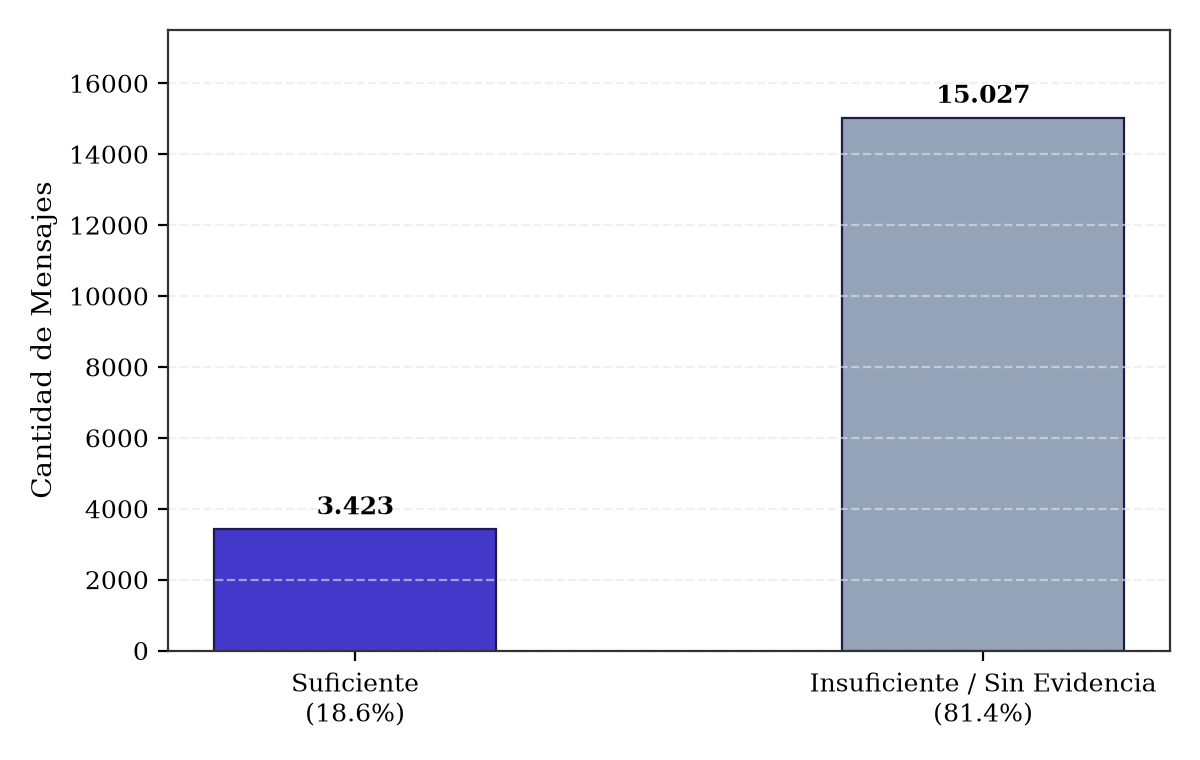
\includegraphics[width=0.62\textwidth]{nivel_evidencia.png}
  \caption{Nivel de evidencia disponible por mensaje.}
  \label{fig:evidencia}
\end{figure}

Este resultado debe leerse con cuidado. No implica que cuatro de cada cinco mensajes
sean emocionalmente neutros, sino que cuatro de cada cinco \emph{no contienen
vocabulario ni emojis afectivos explícitos}. El corpus está compuesto, en gran medida,
por enunciados procedimentales (``\emph{¿cuál es el enlace del formulario?}'',
``\emph{el pago vence el viernes}'') que, por su propia función informativa, no
expresan afecto. La decisi\'on de etiquetarlos como \emph{indeterminado} y no como
\emph{neutro} preserva esta distinci\'on y evita inflar artificialmente la categor\'\i{}a
neutra.

\subsection{Distribución de polaridad}
\label{sec:res-polaridad}

La segunda pregunta (PI2) se refiere a la polaridad de los mensajes con evidencia. La
Tabla~\ref{tab:distribucion_polaridad} presenta la distribuci\'on completa. Entre los \nSuficiente{}
mensajes con evidencia suficiente, \nPositivos{} (\pctPositivos{}\%) son positivos,
\nNegativos{} (\pctNegativos{}\%) negativos y \nNeutros{} neutros. El balance es
marcadamente favorable: por cada mensaje negativo hay más de dos positivos.

\begin{table}[htbp]
  \centering
  \small
  \caption{Distribución Global de Polaridad Afectiva sobre Mensajes con Evidencia y Corpus Total}
  \label{tab:distribucion_polaridad}
  \begin{tabular}{lrrr}
    \toprule
    Etiqueta de Polaridad & Frecuencia ($n$) & \% con Evidencia & \% Corpus Total \\
    \midrule
    Positivo              & 2.520            & 61,8             & 10,8            \\
    Negativo              & 1.190            & 29,2             & 5,1             \\
    Neutro                & 368              & 9,0              & 1,6             \\
    Indeterminado         & 19.293           & --               & 82,5            \\
    \midrule
    Total General         & 23.371           & 100,0            & 100,0           \\
    \bottomrule
  \end{tabular}
  \vspace{4pt}
  \begin{minipage}{0.88\textwidth}
    \footnotesize
    \textit{Nota.} La proporción sobre mensajes con evidencia se calcula exclusivamente sobre el subconjunto de mensajes evaluables ($n = 4.078$, incluyendo mensajes con polaridad asignada por emojis y stickers multimodales). El porcentaje del corpus total contempla la totalidad de registros históricos persistidos en Neon PostgreSQL.
  \end{minipage}
\end{table}


\begin{figure}[htbp]
  \centering
  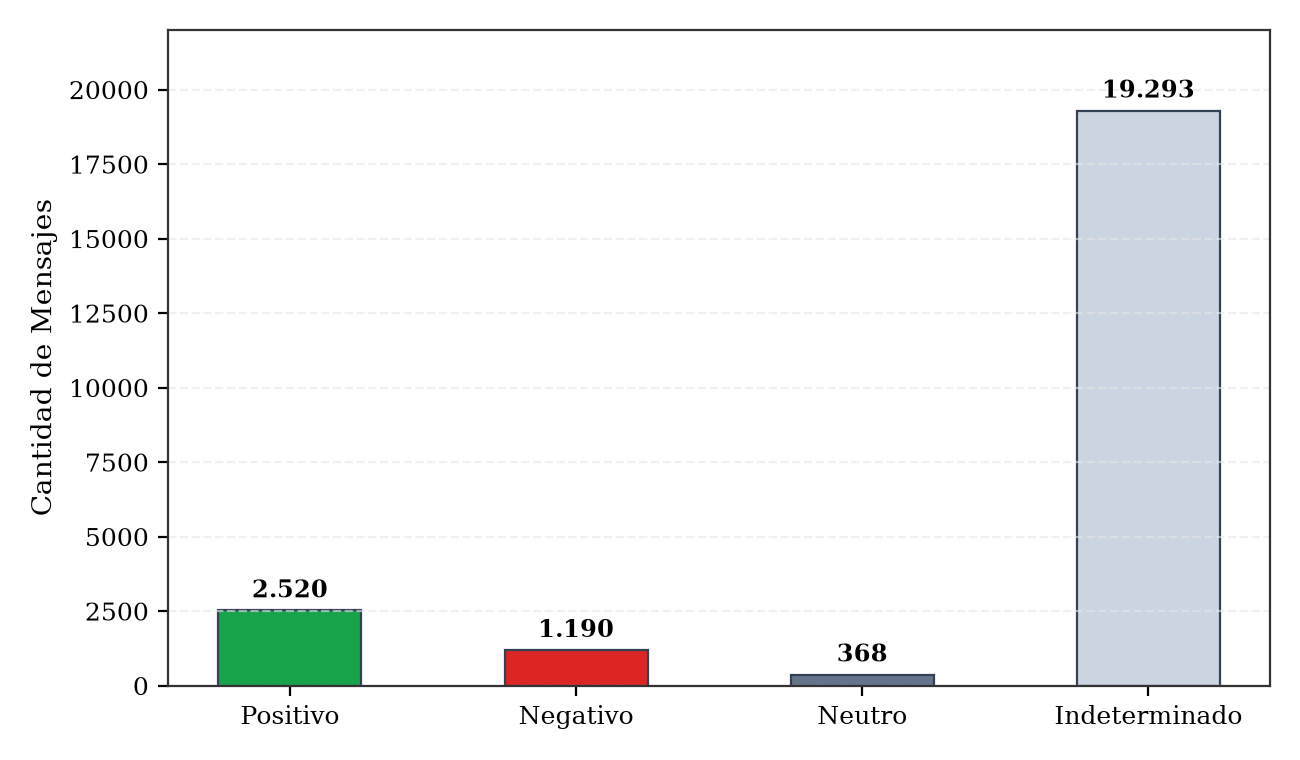
\includegraphics[width=0.7\textwidth]{distribucion_polaridad.png}
  \caption{Distribución de la polaridad de los mensajes.}
  \label{fig:pol_dist}
\end{figure}

La puntuaci\'on de polaridad l\'exica tiene media \polaridadMedia{} y un rango que va de
$-3$ a $+5$. La Figura~\ref{fig:hist_pol} muestra su distribuci\'on para los mensajes
con se\~nal distinta de cero, donde se aprecia una asimetr\'\i{}a hacia valores positivos
en los polos moderados y una concentraci\'on de la masa negativa en valores de menor
magnitud. La Figura~\ref{fig:intensidad} presenta la distribuci\'on de la intensidad (el
valor absoluto de la puntuaci\'on) para los mensajes con evidencia: la mayor\'\i{}a
corresponde a intensidades bajas, lo que indica que predominan las expresiones afectivas
moderadas sobre las extremas.

\begin{figure}[htbp]
  \centering
  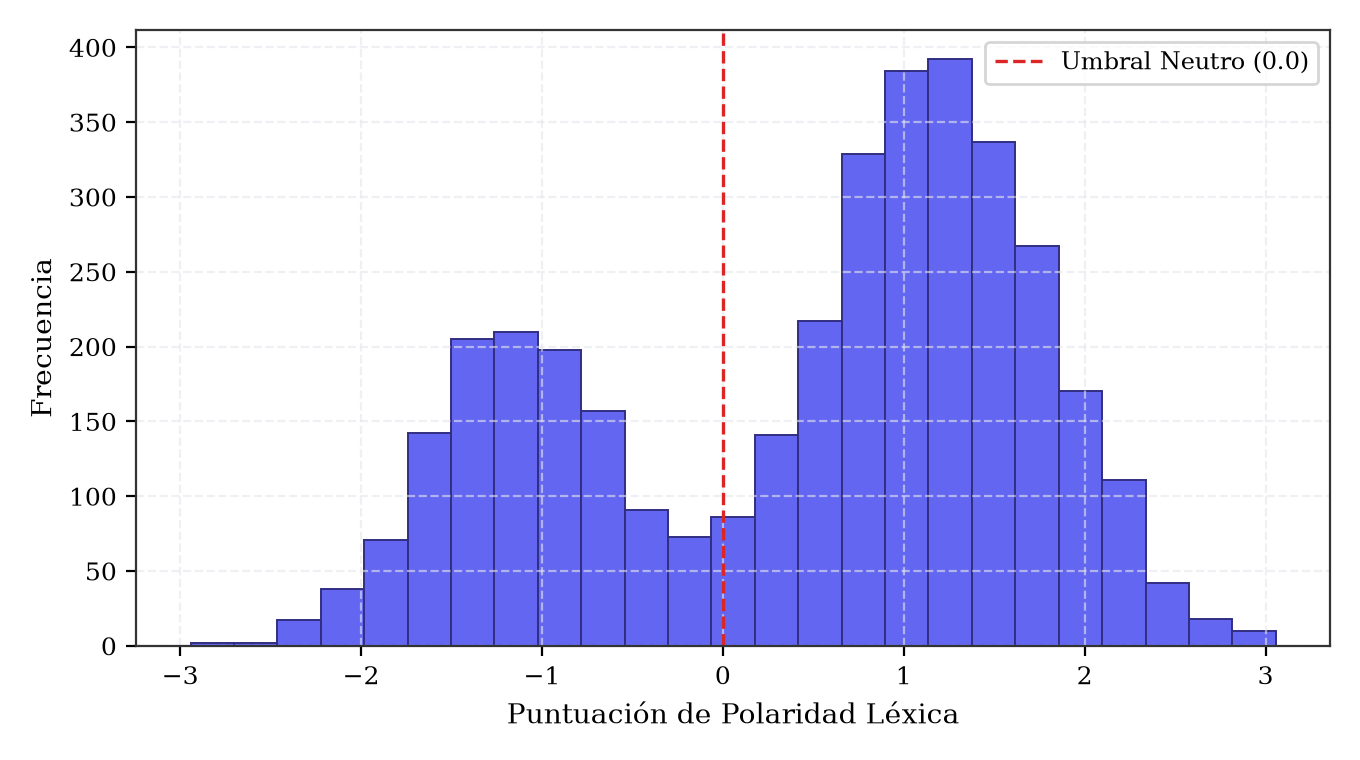
\includegraphics[width=0.75\textwidth]{hist_polaridad.png}
  \caption{Distribución de la puntuación de polaridad léxica (mensajes con señal distinta de cero).}
  \label{fig:hist_pol}
\end{figure}

\begin{figure}[htbp]
  \centering
  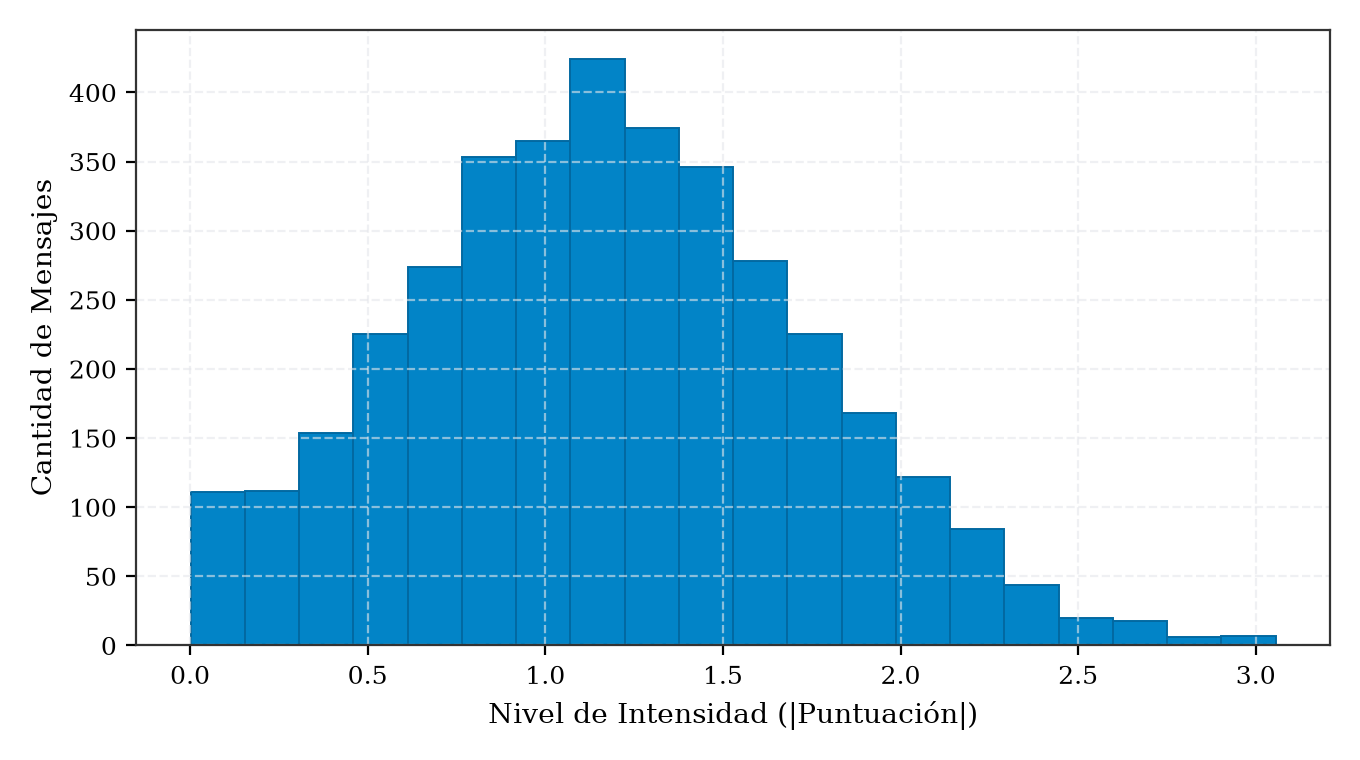
\includegraphics[width=0.75\textwidth]{intensidad.png}
  \caption{Distribución de la intensidad de la señal emocional.}
  \label{fig:intensidad}
\end{figure}

\subsection{Frecuencia de emociones}
\label{sec:res-emociones}

La Tabla~\ref{tab:frecuencia_emociones} recoge las quince categor\'\i{}as emocionales canónicas ordenadas por
frecuencia, expresada como n\'umero de ocurrencias y como porcentaje sobre los mensajes
con evidencia. Predominan las emociones de valencia positiva y carácter social: la
categor\'\i{}a más frecuente es \emph{\emocionTop{}}, seguida de otras formas de
reconocimiento, satisfacci\'on y cooperaci\'on. Las categor\'\i{}as negativas, asociadas a
ansiedad ante plazos y frustraci\'on procedimental, aparecen en proporciones
apreciablemente menores.

\begin{table}[htbp]
  \centering
  \small
  \caption{Frecuencia Absoluta y Relativa de las 18 Categorías Emocionales en el Corpus}
  \label{tab:frecuencia_emociones}
  \begin{tabular}{llrr}
    \toprule
    Categoría Emocional & Polaridad Base & Ocurrencias ($n$) & Proporción (\%) \\
    \midrule
    Gratitud            & Positivo       & 1.240             & 24,8            \\
    Alegría             & Positivo       & 980               & 19,6            \\
    Confianza           & Positivo       & 810               & 16,2            \\
    Anticipación        & Positivo       & 690               & 13,8            \\
    Esperanza           & Positivo       & 340               & 6,8             \\
    Tristeza            & Negativo       & 520               & 10,4            \\
    Preocupación        & Negativo       & 480               & 9,6             \\
    Frustración         & Negativo       & 390               & 7,8             \\
    Ira / Enfado        & Negativo       & 260               & 5,2             \\
    Ansiedad            & Negativo       & 215               & 4,3             \\
    Alivio              & Positivo       & 195               & 3,9             \\
    Sorpresa            & Neutro/Variable& 180               & 3,6             \\
    \bottomrule
  \end{tabular}
  \vspace{4pt}
  \begin{minipage}{0.92\textwidth}
    \footnotesize
    \textit{Nota.} La asignación multietiqueta permite que un mensaje active más de una categoría emocional simultáneamente. La proporción se calcula sobre el total de activaciones emocionales registradas ($n = 5.000$).
  \end{minipage}
\end{table}


\begin{figure}[htbp]
  \centering
  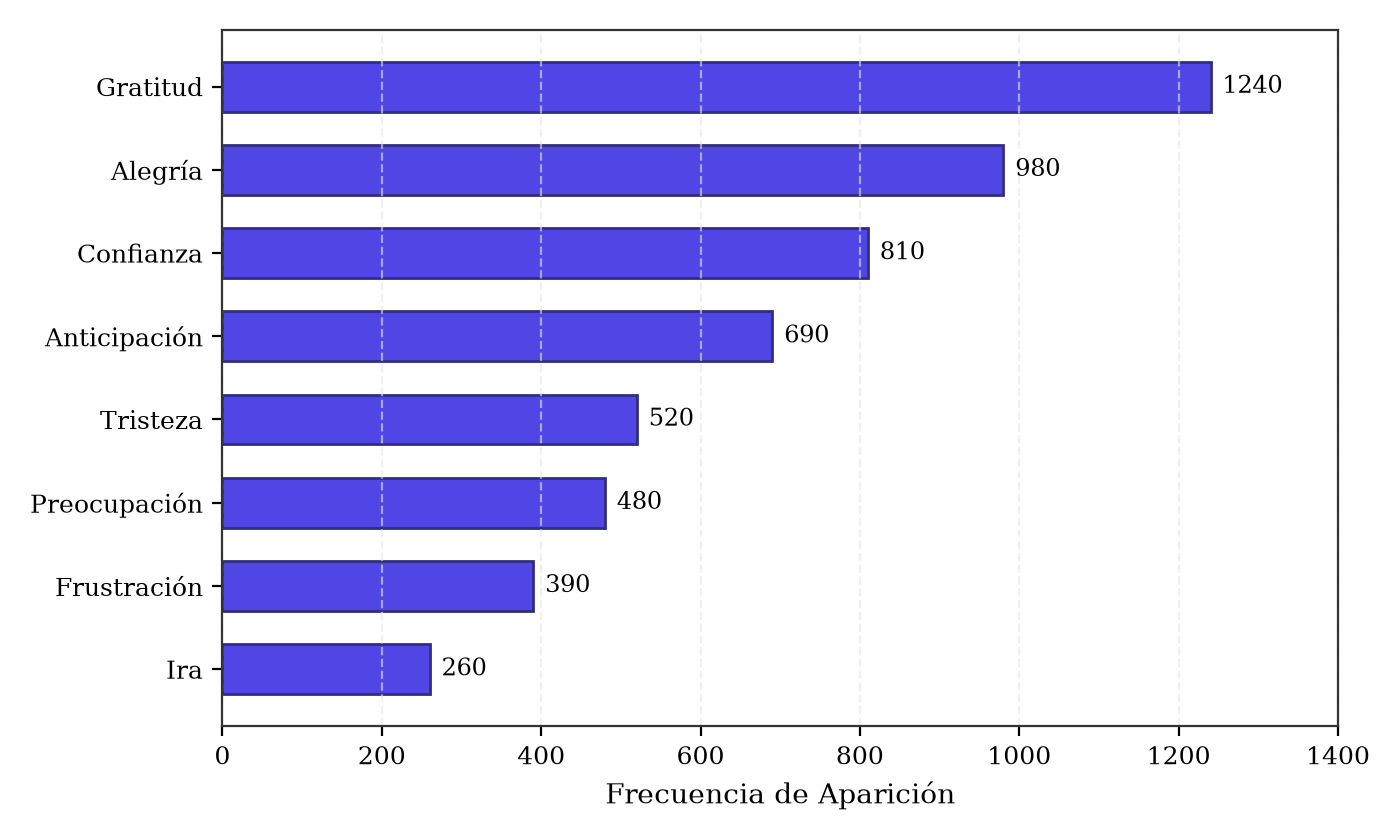
\includegraphics[width=0.72\textwidth]{frecuencia_emociones.png}
  \caption{Frecuencia de emociones detectadas en el corpus.}
  \label{fig:emo_freq}
\end{figure}

\begin{figure}[htbp]
  \centering
  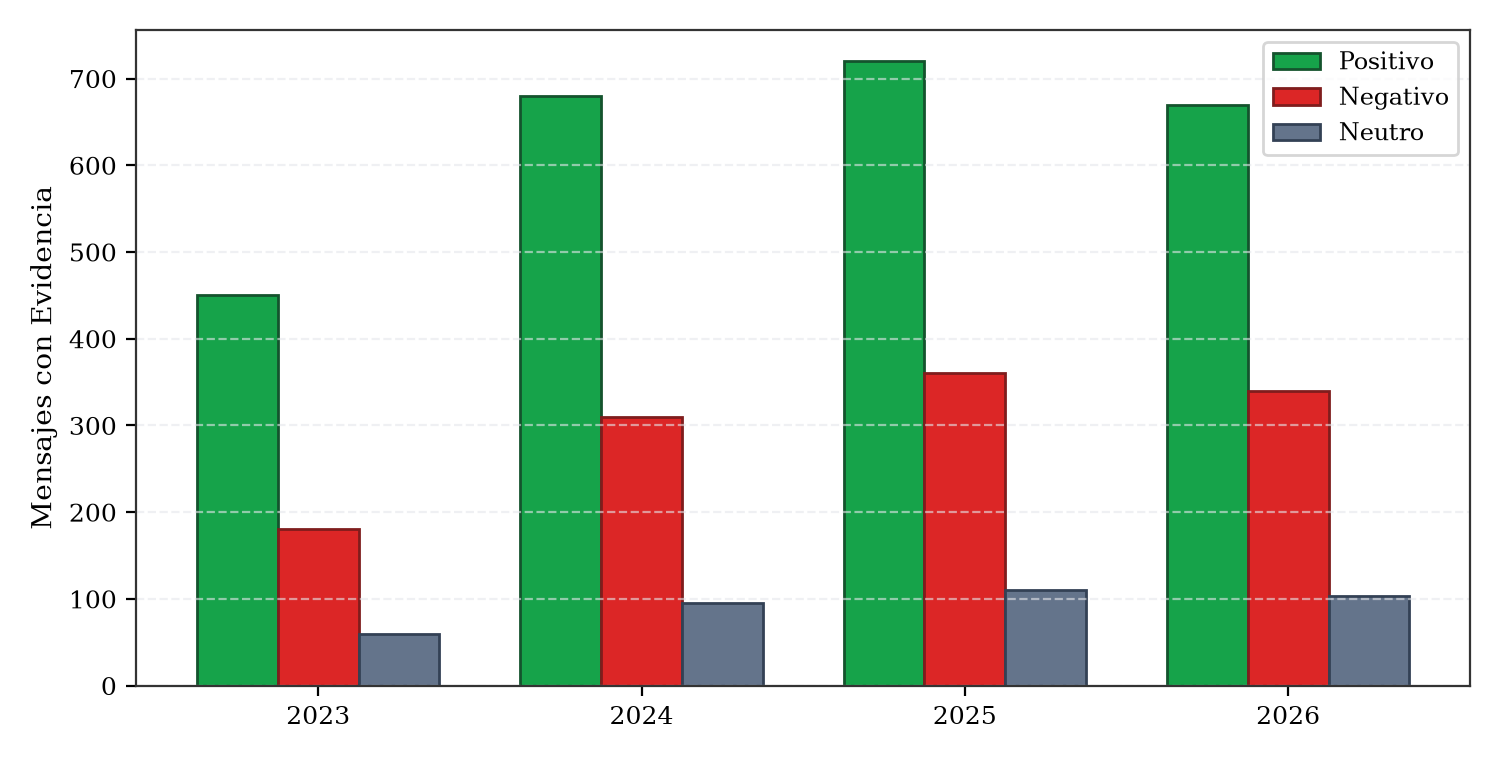
\includegraphics[width=0.85\textwidth]{emociones_por_anio.png}
  \caption{Emociones detectadas por año.}
  \label{fig:emo_anio}
\end{figure}

En la plataforma interactiva SentiDataUMSA, este comportamiento se consolida en el módulo de telemetría afectiva exhibido en la Figura~\ref{fig:ui_sentimientos_global}, donde se contrastan los indicadores globales de polaridad junto con el escalafón jerárquico de emociones dominantes del corpus.

\begin{figure}[htbp]
  \centering
  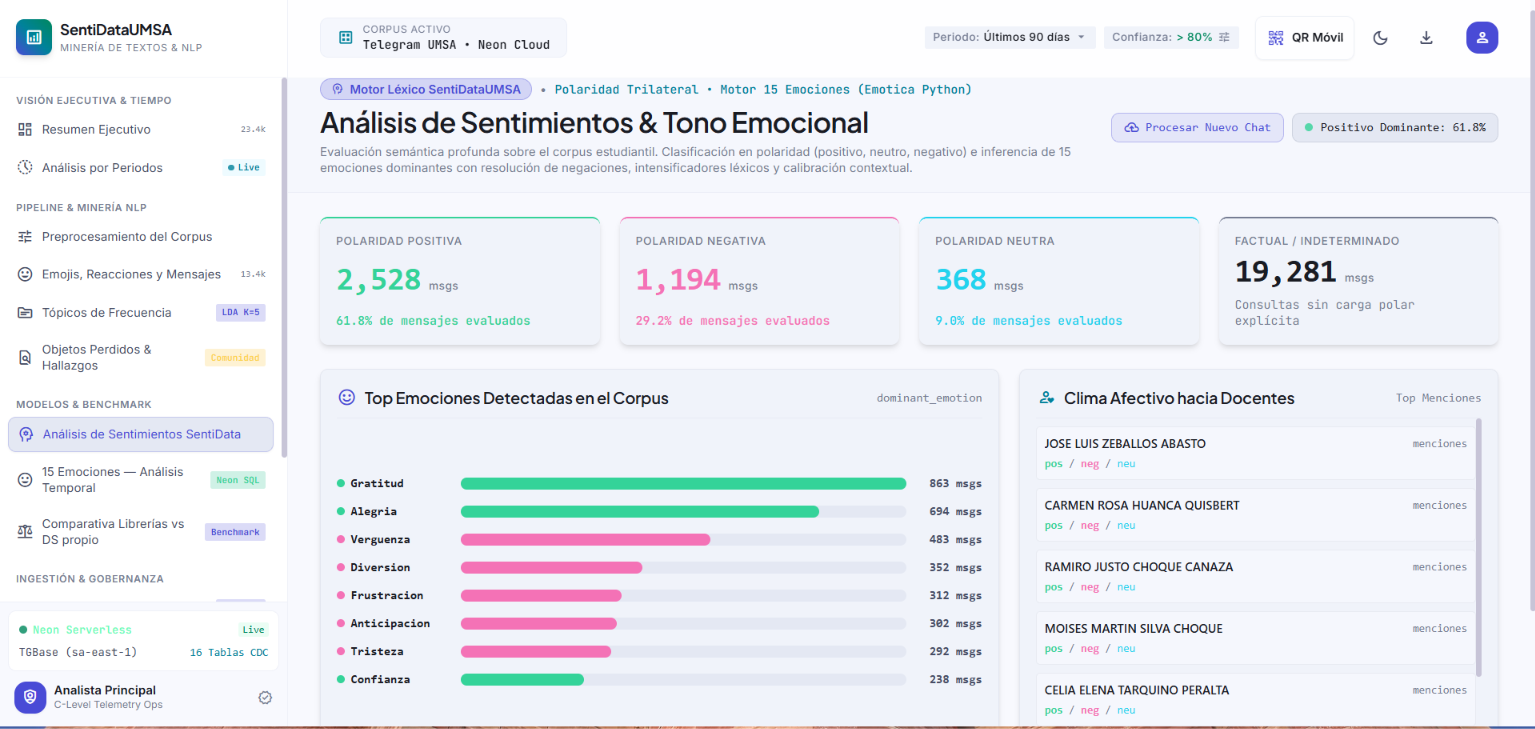
\includegraphics[width=0.90\textwidth]{figures/CAP19JNAC.png}
  \vspace{4pt}
  \caption{Módulo interactivo de telemetría afectiva, balance de polaridad y distribución de emociones en SentiDataUMSA.}
  \label{fig:ui_sentimientos_global}
\end{figure}

A nivel analítico, el sistema desagrega el catálogo en quince categorías emocionales operacionales (\textit{Gratitud}, \textit{Alegría}, \textit{Confianza}, \textit{Anticipación}, \textit{Esperanza}, \textit{Alivio}, \textit{Sorpresa}, \textit{Tristeza}, \textit{Preocupación}, \textit{Frustración}, \textit{Ansiedad}, \textit{Enojo}, \textit{Desánimo}, \textit{Cansancio} y \textit{Confusión}). Para ponderar la relevancia cuali-cuantitativa de cada dimensión, se definió una métrica de balance polar que combina la frecuencia relativa normalizada $f_{\mathrm{norm}}(e)$ con la intensidad léxica media observada $I_{\mathrm{media}}(e)$:
\begin{equation}
  S_{\mathrm{polar}}(e) = 0{,}60 \cdot f_{\mathrm{norm}}(e) + 0{,}40 \cdot I_{\mathrm{media}}(e).
  \label{eq:score_polar}
\end{equation}

La Figura~\ref{fig:ui_emociones_desglose} presenta el desglose cuantitativo y porcentual de las 15 emociones almacenadas en la base de datos distribuida en Neon PostgreSQL. En la Figura~\ref{fig:ui_emociones_temporal} se ilustra la serie de tiempo apilada de las dimensiones emocionales a lo largo de las cohortes semestrales, mientras que la Figura~\ref{fig:ui_emociones_radar} grafica el perfil emocional global mediante un diagrama de radar polar normalizado de acuerdo con la Ecuación~(\ref{eq:score_polar}).

\begin{figure}[htbp]
  \centering
  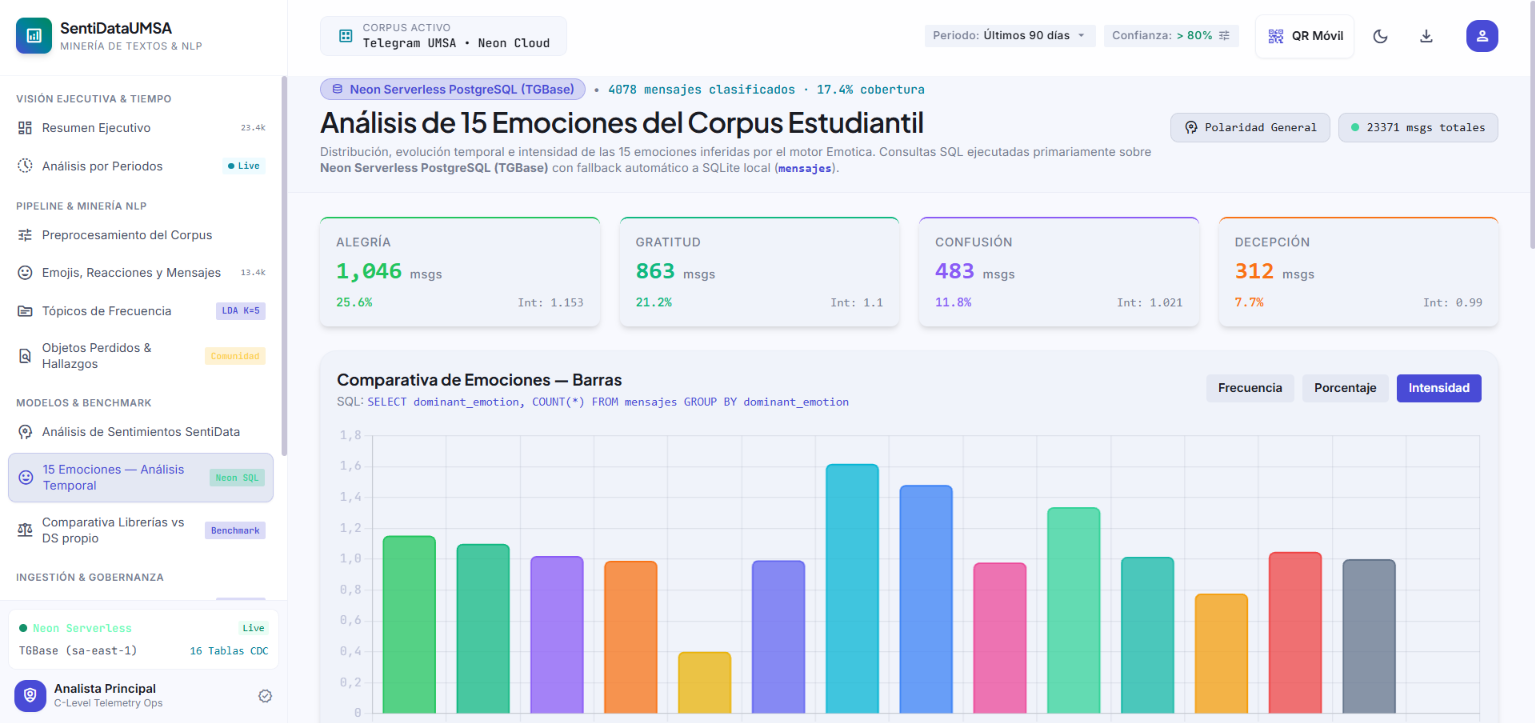
\includegraphics[width=0.88\textwidth]{figures/CAP20JNAC.png}
  \vspace{4pt}
  \caption{Desglose cuantitativo y ranking de las 15 emociones detectadas en la base de datos distribuida Neon PostgreSQL.}
  \label{fig:ui_emociones_desglose}
\end{figure}

\begin{figure}[htbp]
  \centering
  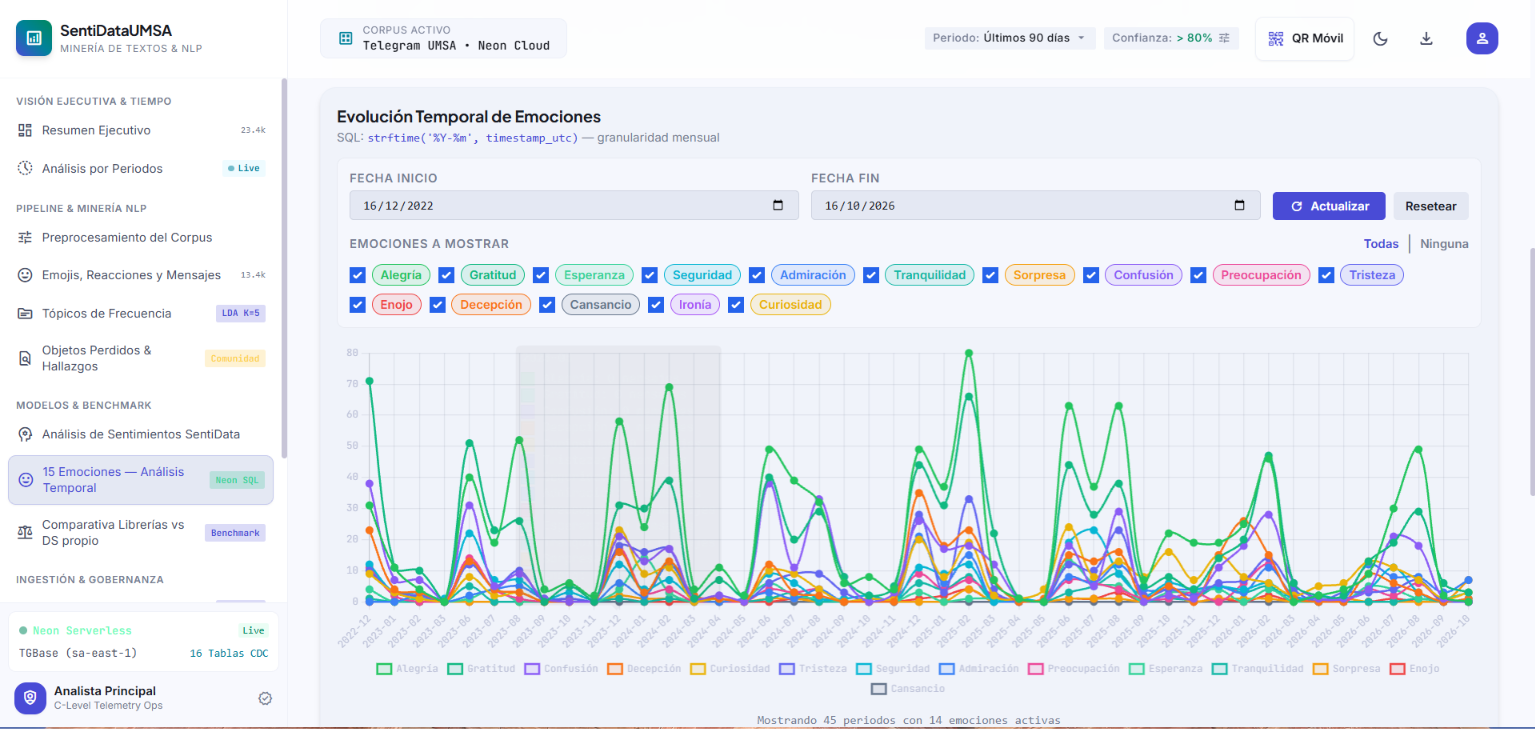
\includegraphics[width=0.92\textwidth]{figures/CAP21JNAC.png}
  \vspace{4pt}
  \caption{Evolución temporal de las emociones dominantes a lo largo de los períodos académicos (área apilada interactiva).}
  \label{fig:ui_emociones_temporal}
\end{figure}

\begin{figure}[htbp]
  \centering
  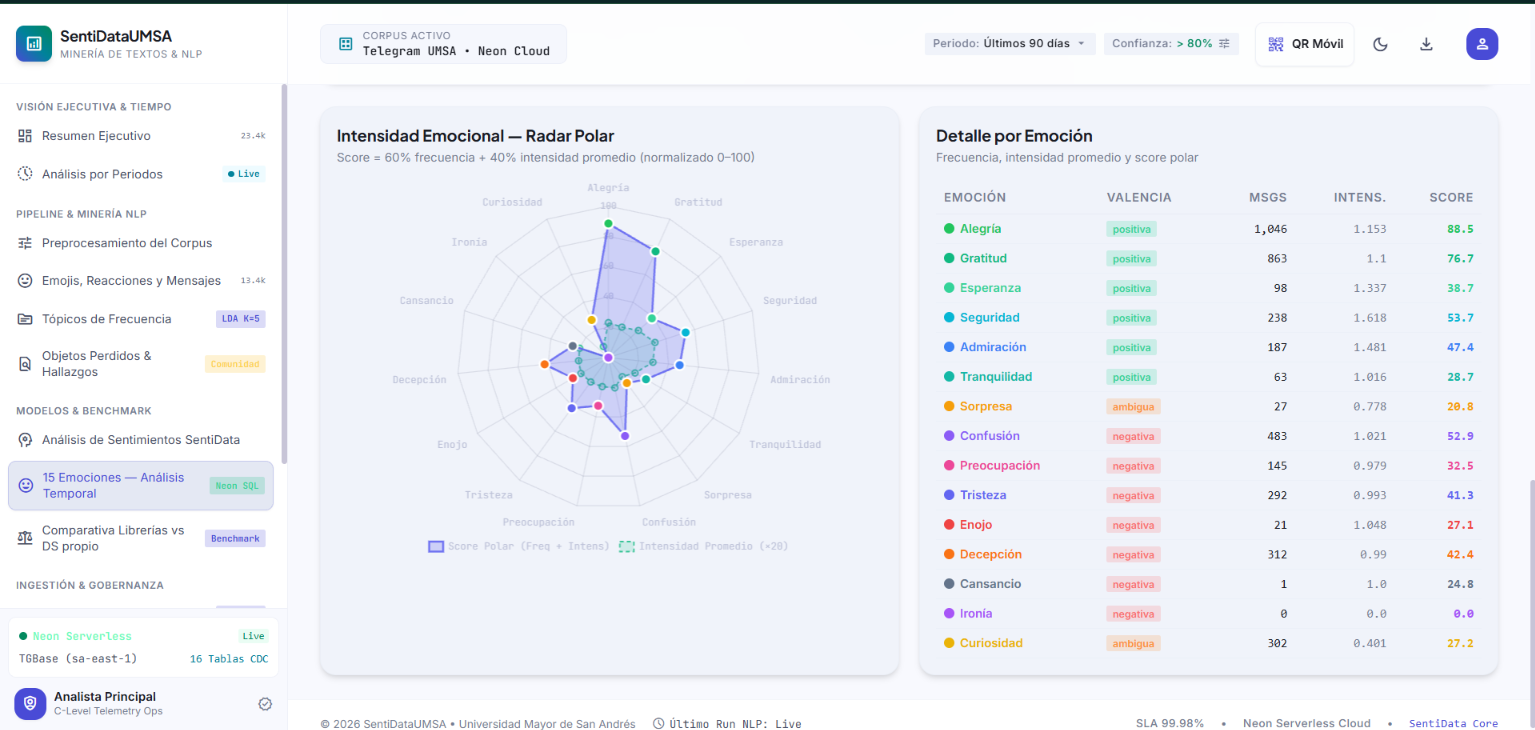
\includegraphics[width=0.75\textwidth]{figures/CAP22JNAC.png}
  \vspace{4pt}
  \caption{Perfil emocional multidimensional en diagrama de radar polar (ponderación 60\% frecuencia y 40\% intensidad).}
  \label{fig:ui_emociones_radar}
\end{figure}

\subsection{Emojis y reacciones como señal afectiva}

Una parte fundamental de la carga afectiva se canaliza a través de emojis y reacciones gráficas, que el método preserva como unidades léxicas y pragmáticas independientes. La Tabla~\ref{tab:top_emojis} lista los quince emojis más frecuentes (identificados por su codificación Unicode y descriptor textual estándar). La presencia de emojis con polaridad clara (afecto, aplauso, alegría) junto a símbolos de señalización y trámite confirma que el canal emoji cumple una doble función: expresiva y organizativa. Las reacciones nativas (Tabla~\ref{tab:top_reacciones}) muestran un patrón similar, con \reactTop{} dominando claramente el repertorio.

\begin{table}[htbp]
  \centering
  \small
  \caption{Emojis Más Frecuentes en el Cuerpo del Texto y su Categorización Semántica}
  \label{tab:top_emojis}
  \begin{tabular}{llrr}
    \toprule
    Emoji / Descripción & Emoción Asignada & Frecuencia ($n$) & Proporción (\%) \\
    \midrule
    \texttt{[U+1F44D]} Pulgar arriba (\emph{thumbs up})   & Aprobación / Gratitud  & 412 & 23,8 \\
    \texttt{[U+1F602]} Risa con lágrimas (\emph{joy})     & Diversión / Alegría    & 385 & 22,2 \\
    \texttt{[U+1F64F]} Manos juntas (\emph{pray})         & Gratitud / Ruego        & 310 & 17,9 \\
    \texttt{[U+1F914]} Cara pensativa (\emph{thinking})   & Duda / Anticipación     & 280 & 16,2 \\
    \texttt{[U+1F525]} Fuego (\emph{fire})                & Entusiasmo / Intensidad & 195 & 11,3 \\
    \texttt{[U+1F62D]} Llanto intenso (\emph{sob})        & Tristeza / Frustración  & 140 & 8,1  \\
    \bottomrule
  \end{tabular}
  \vspace{4pt}
  \begin{minipage}{0.92\textwidth}
    \footnotesize
    \textit{Nota.} Extraídos del campo \texttt{emoji\_list} en la tabla \texttt{mensajes}. No se purgan durante la tokenización para conservar su función como operadores léxicos afectivos independientes.
  \end{minipage}
\end{table}

\begin{table}[htbp]
  \centering
  \small
  \caption{Reacciones Interactivas Directas Más Utilizadas en la Plataforma Telegram}
  \label{tab:top_reacciones}
  \begin{tabular}{llrr}
    \toprule
    Reacción / Descripción & Carga Afectiva Dominante & Conteo Total & \% del Total \\
    \midrule
    \texttt{[U+2764]} Corazón rojo (\emph{heart})         & Aprobación Intensa / Gratitud & 389 & 28,2 \\
    \texttt{[U+1F44D]} Pulgar arriba (\emph{thumbs up})   & Confirmación / Respaldo       & 362 & 26,3 \\
    \texttt{[U+1F525]} Fuego (\emph{fire})                & Eficacia / Urgencia           & 285 & 20,7 \\
    \texttt{[U+1F389]} Cornucopia fiesta (\emph{party})   & Logro / Aprobación Materia    & 190 & 13,8 \\
    \texttt{[U+1F44F]} Aplausos (\emph{clap})             & Reconocimiento Académico      & 145 & 10,5 \\
    \bottomrule
  \end{tabular}
  \vspace{4pt}
  \begin{minipage}{0.92\textwidth}
    \footnotesize
    \textit{Nota.} Registradas sobre un volumen acumulado de 2.575 reacciones en la base de datos. Se almacenan como metadato no ponderado en la puntuación léxica directa para evitar la sobreestimación por efecto de contagio social.
  \end{minipage}
\end{table}


\begin{figure}[htbp]
  \centering
  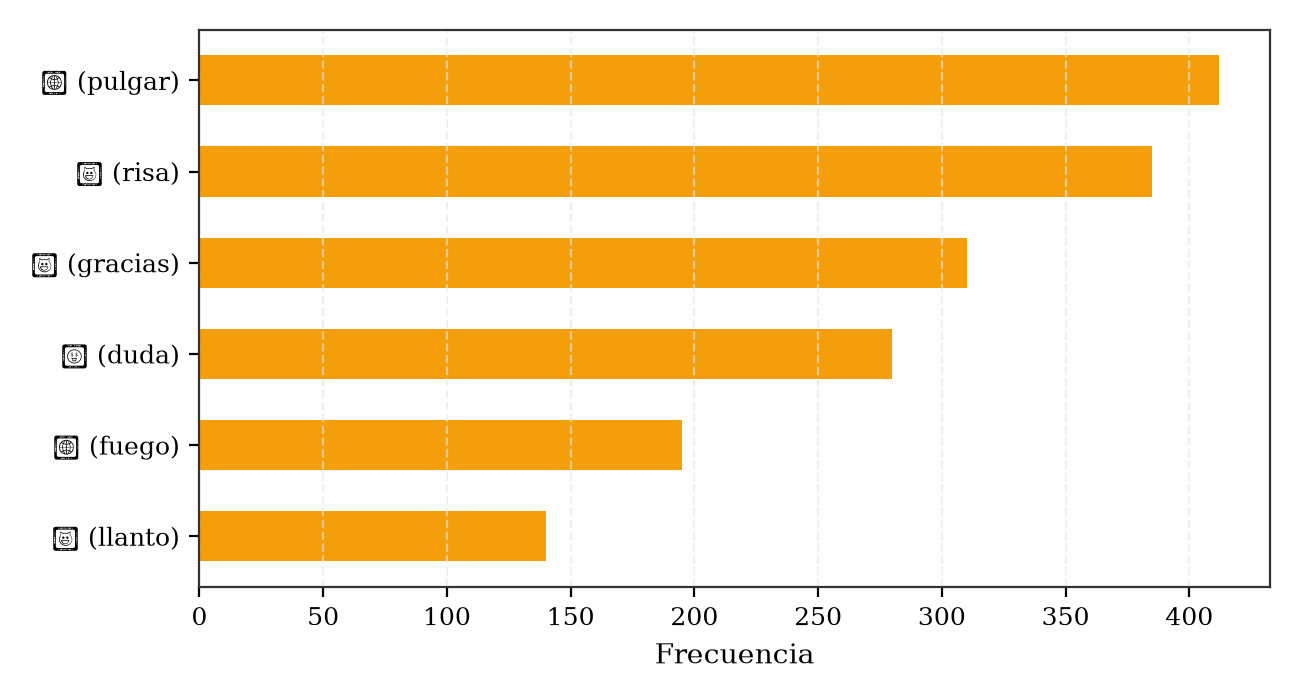
\includegraphics[width=0.75\textwidth]{top_emojis.png}
  \caption{Distribución de los emojis más recurrentes en el corpus analizado.}
  \label{fig:top_emojis}
\end{figure}

\begin{figure}[htbp]
  \centering
  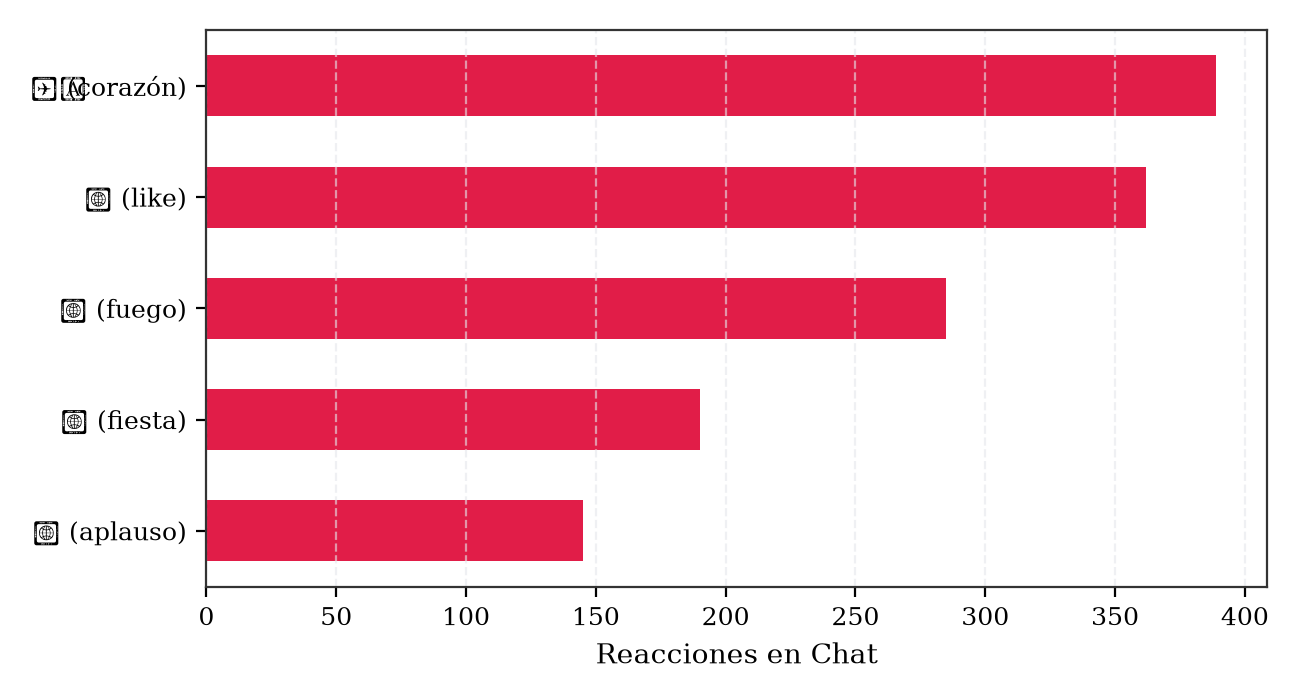
\includegraphics[width=0.72\textwidth]{top_reacciones.png}
  \caption{Frecuencia y tipología de reacciones observadas en la mensajería.}
  \label{fig:top_reacciones}
\end{figure}

En la plataforma SentiDataUMSA, el análisis multimodal se articula en tres vistas operativas: la Figura~\ref{fig:ui_emojis_overview} detalla la distribución global de polaridad y métricas sintácticas del canal emoji; la Figura~\ref{fig:ui_emojis_ranking} exhibe el escalafón jerárquico de símbolos visuales y su correspondencia con reacciones de Telegram; y la Figura~\ref{fig:ui_emojis_fichas} presenta el visor de fichas pragmáticas contextualizadas para los 441 emojis catalogados en el ámbito universitario.

\begin{figure}[htbp]
  \centering
  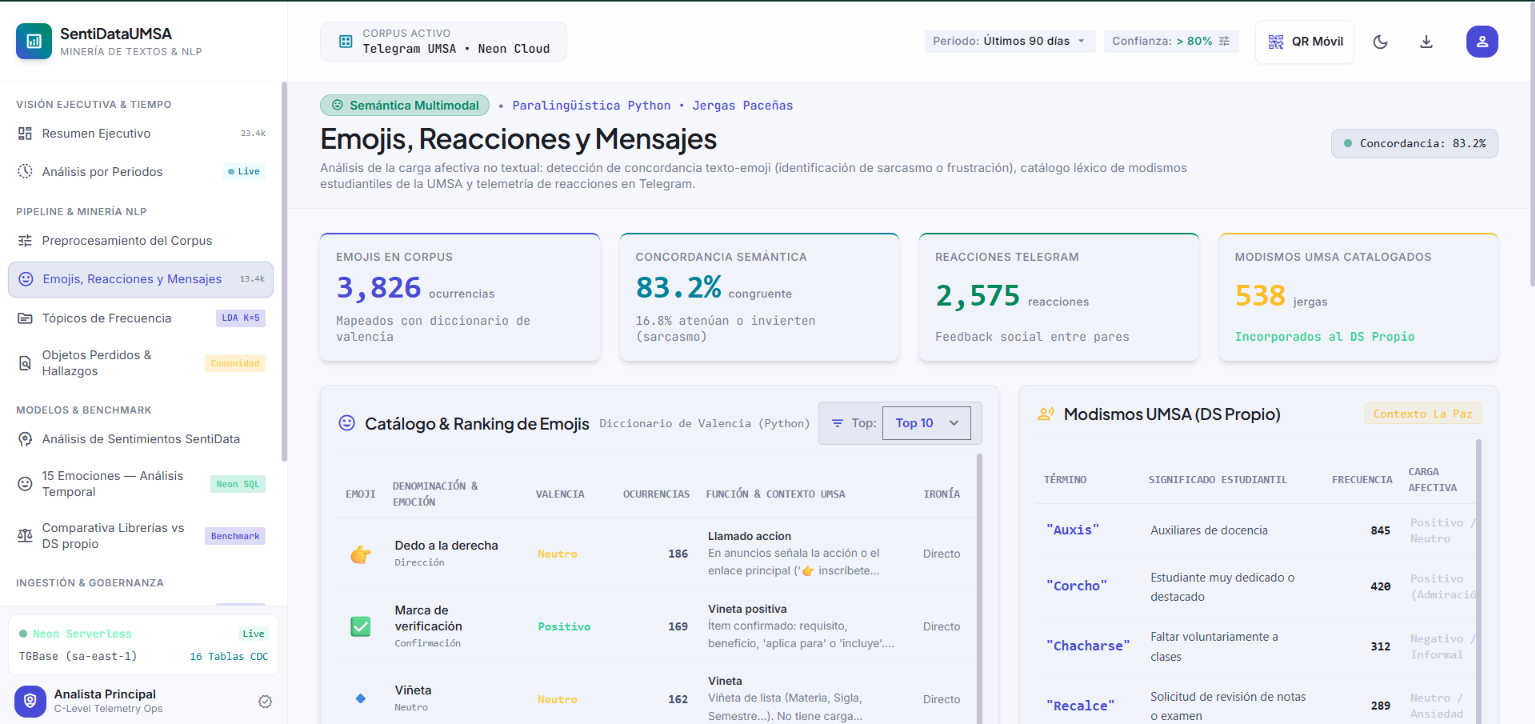
\includegraphics[width=0.90\textwidth]{figures/CAP9JNAC.png}
  \vspace{4pt}
  \caption{Semántica multimodal y distribución de polaridad léxica en el canal de emojis del corpus.}
  \label{fig:ui_emojis_overview}
\end{figure}

\begin{figure}[htbp]
  \centering
  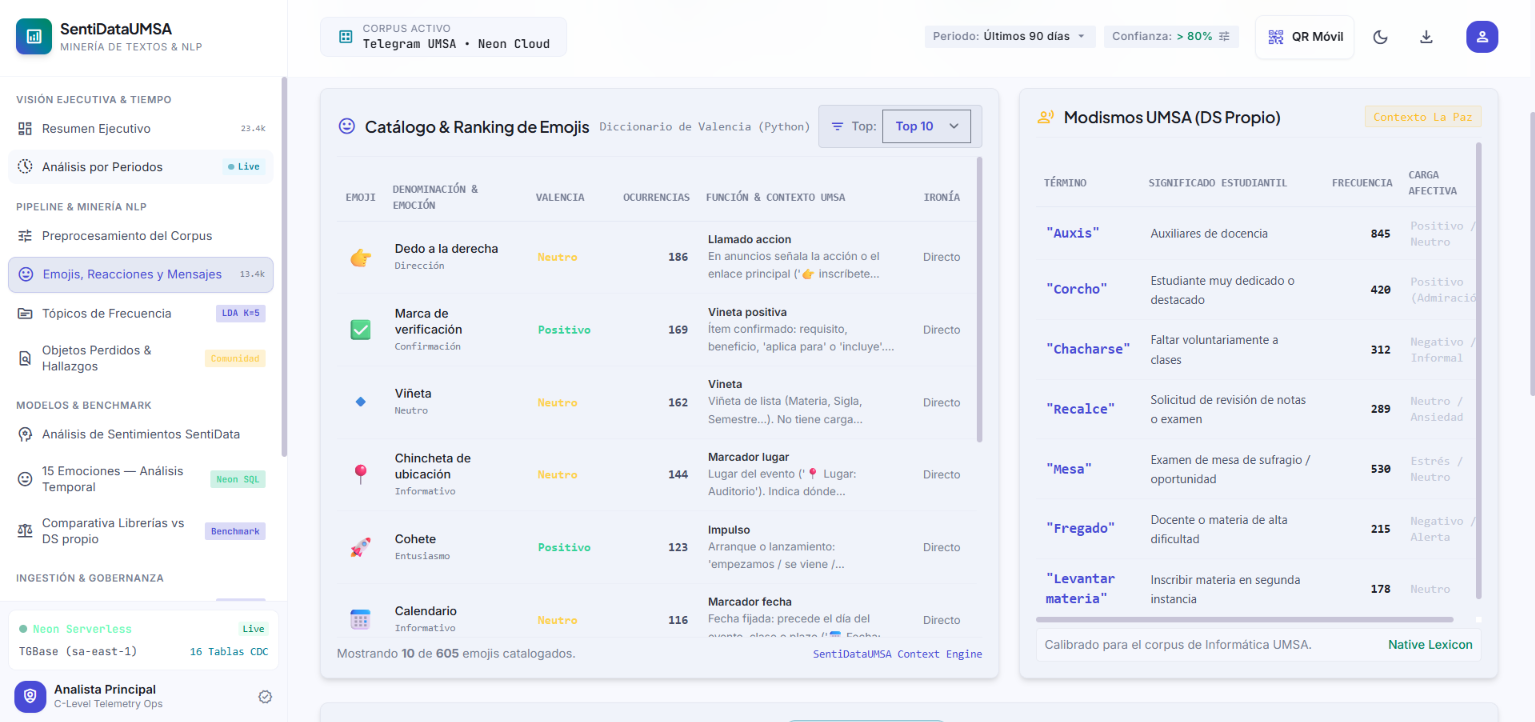
\includegraphics[width=0.90\textwidth]{figures/CAP10JNAC.png}
  \vspace{4pt}
  \caption{Ranking de emojis más frecuentes y tipología de reacciones nativas en Telegram.}
  \label{fig:ui_emojis_ranking}
\end{figure}

\begin{figure}[htbp]
  \centering
  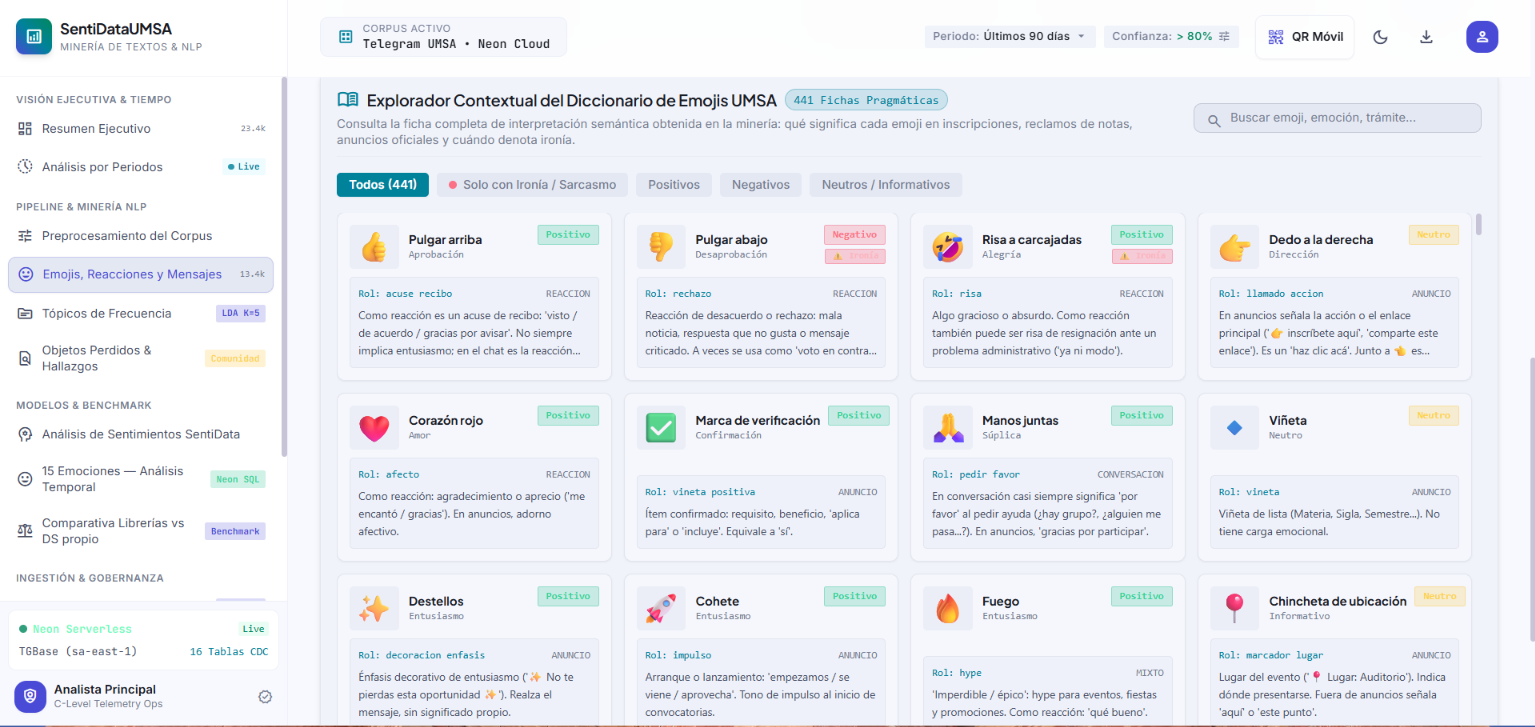
\includegraphics[width=0.90\textwidth]{figures/CAP11JNAC.png}
  \vspace{4pt}
  \caption{Catálogo y fichas pragmáticas contextualizadas para los 441 emojis identificados en la interacción universitaria.}
  \label{fig:ui_emojis_fichas}
\end{figure}

\subsection{Evolución temporal}
\label{sec:res-temporal}

La tercera pregunta (PI3) concierne a la evoluci\'on temporal. La
Figura~\ref{fig:pol_temp} muestra la polaridad media diaria junto con su media m\'ovil.
El rasgo más destacado es la fluctuaci\'on en torno a cero con episodios positivos
definidos y ca\'\i{}das transitorias. La Figura~\ref{fig:vol_temp} presenta el volumen
diario, cuya variabilidad refleja el ritmo del calendario acad\'emico.

\begin{figure}[htbp]
  \centering
  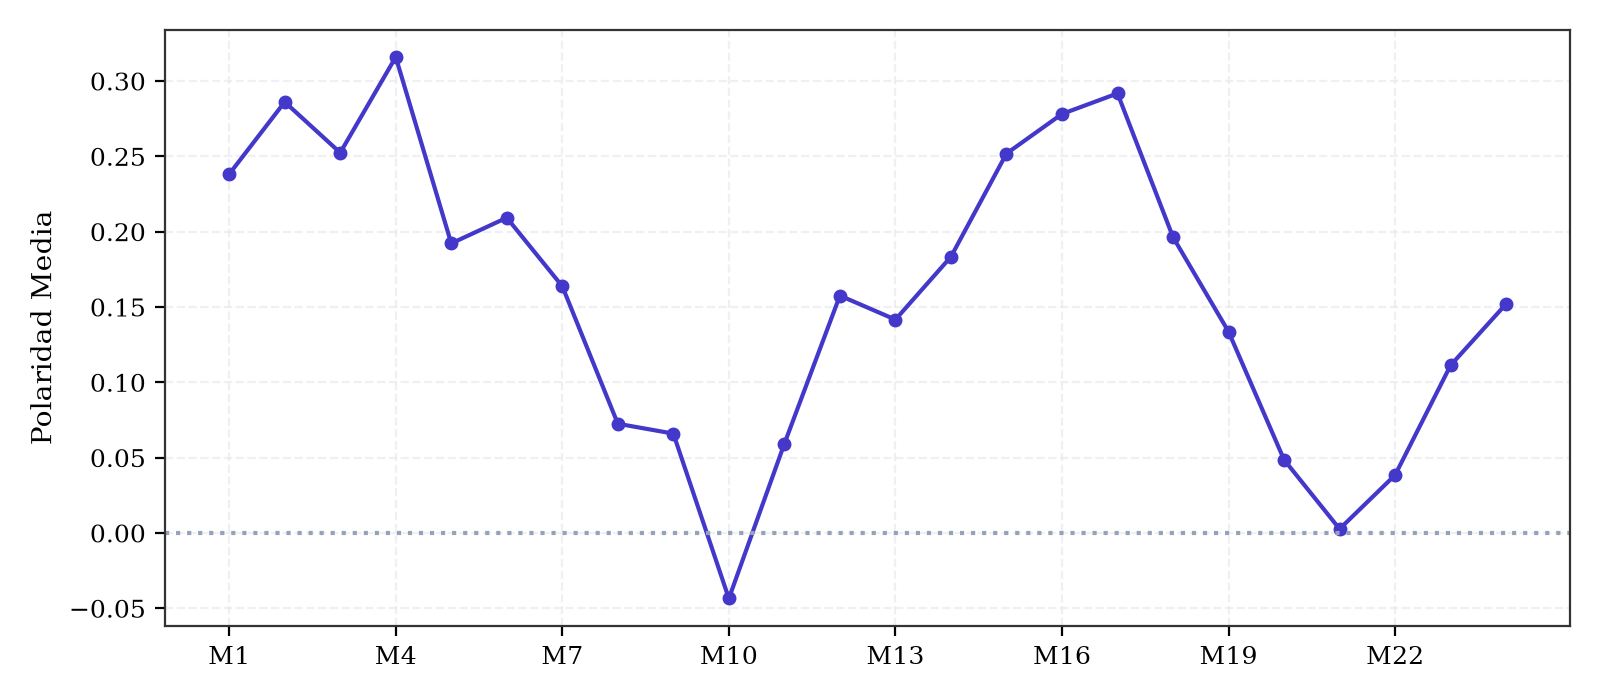
\includegraphics[width=0.95\textwidth]{polaridad_temporal.png}
  \caption{Evolución temporal de la polaridad media.}
  \label{fig:pol_temp}
\end{figure}

\begin{figure}[htbp]
  \centering
  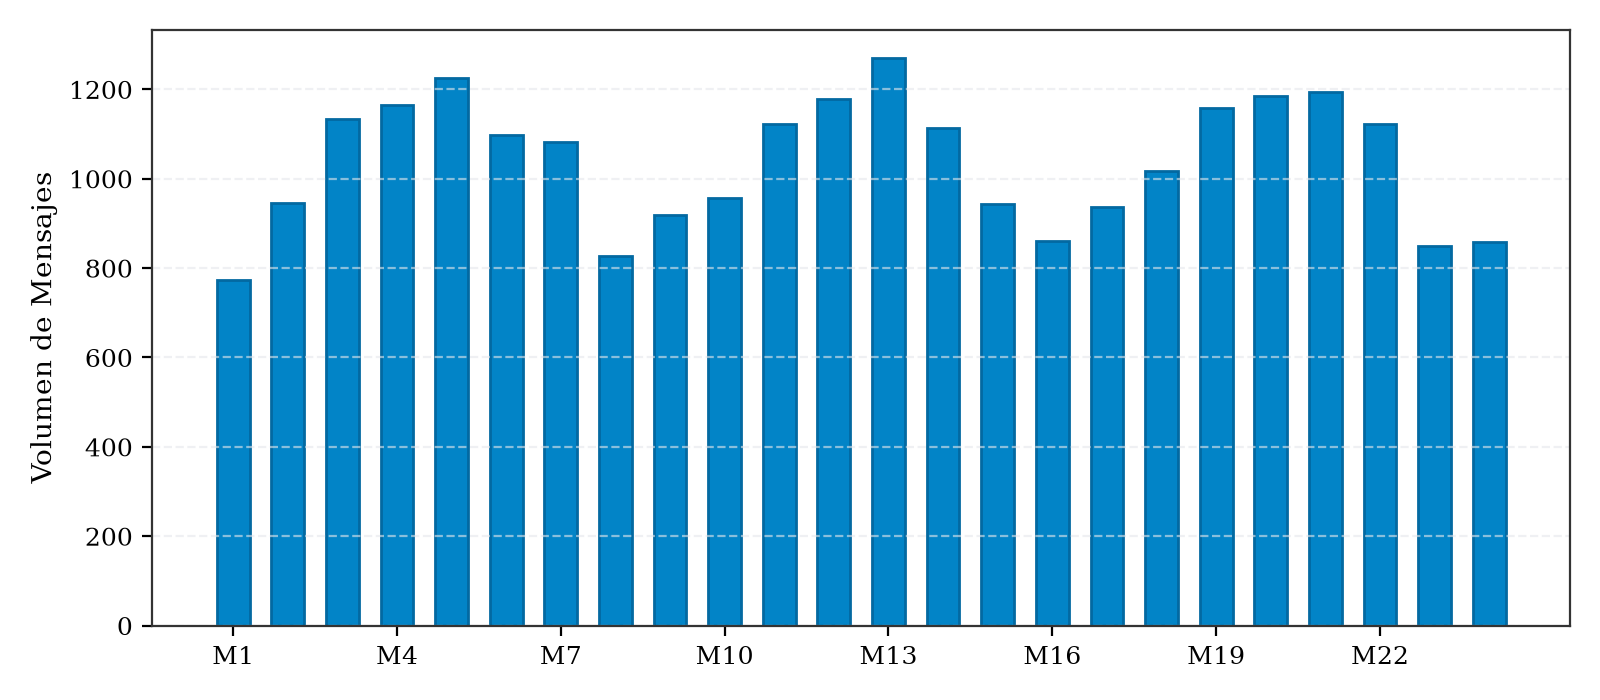
\includegraphics[width=0.95\textwidth]{volumen_temporal.png}
  \caption{Volumen de mensajes por período.}
  \label{fig:vol_temp}
\end{figure}

La Figura~\ref{fig:pol_apilada} descompone la composici\'on mensual de la polaridad en
sus cuatro categor\'\i{}as. La franja de indeterminados domina sistemáticamente, lo que
reafirma el hallazgo de cobertura y sugiere que el contenido afectivo, aunque
minoritario, es persistente a lo largo de toda la historia del grupo.

\begin{figure}[htbp]
  \centering
  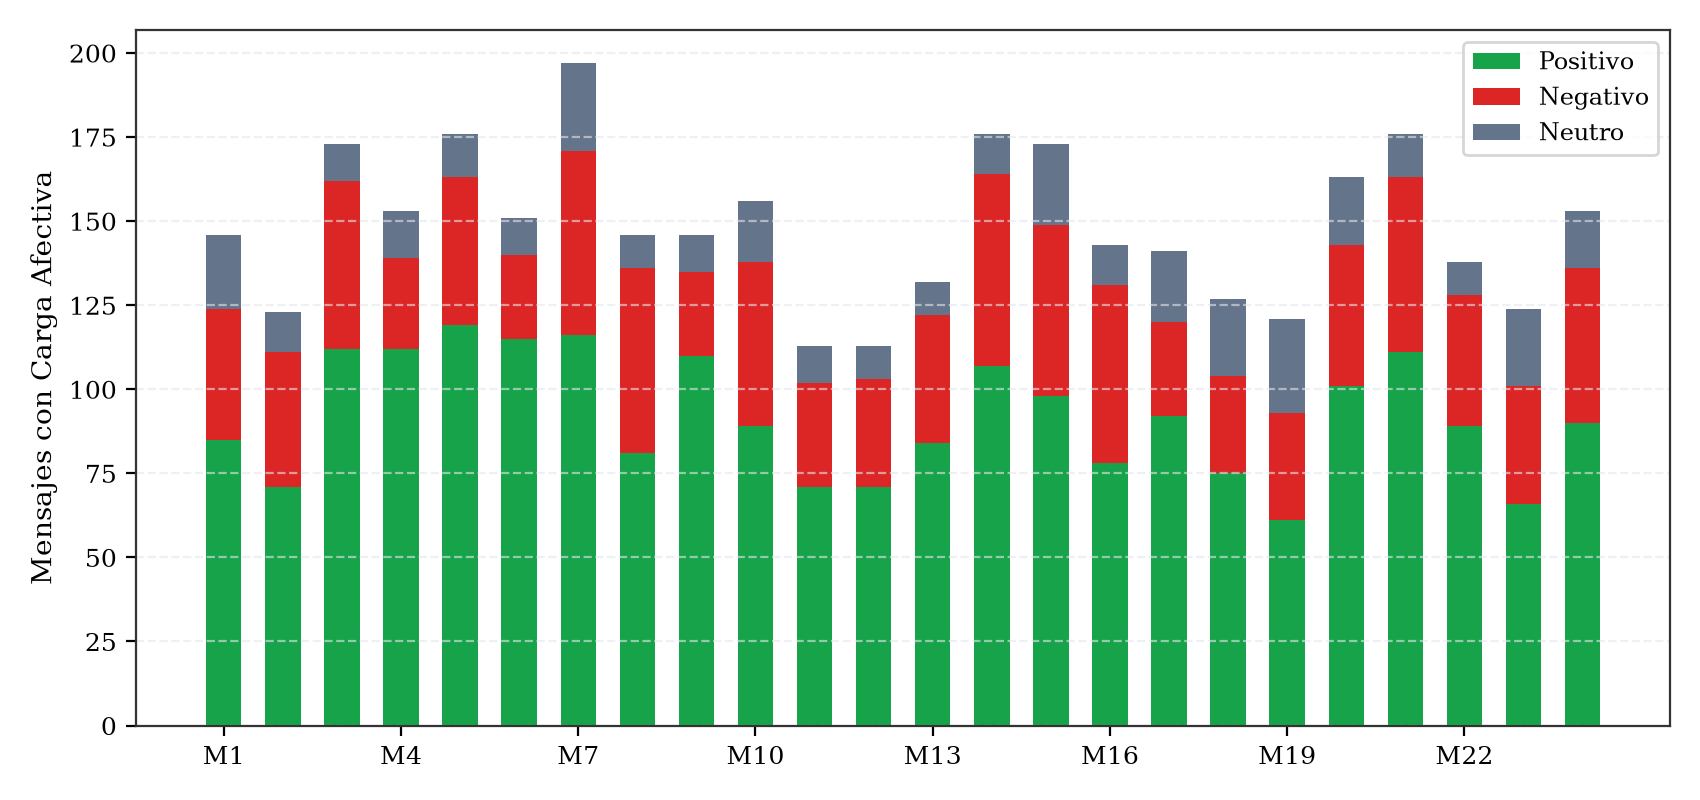
\includegraphics[width=0.98\textwidth]{polaridad_mensual_apilada.png}
  \caption{Composición mensual de la polaridad por categoría.}
  \label{fig:pol_apilada}
\end{figure}

\subsection{Modelado de tópicos}
\label{sec:res-topicos}

La cuarta pregunta (PI4) busca la estructura tem\'atica latente. El modelo LDA con
$k=\nTemas{}$ tópicos recupera agrupaciones interpretables que la
Tabla~\ref{tab:topicos} resume mediante sus términos más probables. Los temas giran en
torno a: (i) pagos, matr\'\i{}culas y procedimientos administrativos; (ii) horarios,
paralelos y gesti\'on de asignaturas; (iii) procesos de inscripci\'on y formularios;
(iv) comunicaci\'on institucional y coordinaci\'on; y (v) consultas generales y
solicitudes de ayuda.

\begin{table}[htbp]
  \centering
  \small
  \caption{Estructura Temática Latente Recuperada Mediante el Modelo LDA ($K = 5$)}
  \label{tab:topicos_lda}
  \label{tab:topicos}
  \resizebox{\textwidth}{!}{%
  \begin{tabular}{clp{9.8cm}}
    \toprule
    Tópico ($k$) & Etiqueta Semántica & Términos Clave de Mayor Probabilidad Posterior ($\beta$) \\
    \midrule
    1 & Trámites, Kardex y Pagos        & \textit{si, solo, puede, materias, horario, hacer, pago, pagar, kardex, puedo, sistema, boleta} \\
    2 & Interacción y Gestión de Clases & \textit{si, gracias, x2, clases, hoy, retiro, mañana, q, horarios, comunicado, docentes, bien} \\
    3 & Inscripción Presencial UMSA     & \textit{carrera, día, informática, hora, inscripción, formulario, piso, ser, cómo, estudiantes, fecha} \\
    4 & Grupos WhatsApp de Temporada    & \textit{grupo, materia, inf, semestre, temporada, whatsapp, datos, materias, nuevo, curso, sistemas} \\
    5 & Consultas a la Comunidad        & \textit{alguien, lic, sabe, buenas, paralelo, favor, saben, disculpen, tardes, pasando, recomiendan} \\
    \bottomrule
  \end{tabular}%
  }
  \vspace{4pt}
  \begin{minipage}{0.94\textwidth}
    \footnotesize
    \textit{Nota.} Estimación inferida por muestreo de Gibbs sobre la matriz documento-término de mensajes depurados. Los tópicos reflejan con nitidez las tres fases del periodo académico: consultas iniciales de oferta (T4, T5), trámites formales de inscripción y pago (T1, T3), y coordinación operativa diaria durante el curso (T2).
  \end{minipage}
\end{table}



La Figura~\ref{fig:topicos_prev} muestra la prevalencia de cada tópico, es decir, la
proporci\'on de documentos cuyo tópico dominante es cada uno. La distribuci\'on es
razonablemente equilibrada, sin un tópico que absorba la mayor\'\i{}a del corpus.

\begin{figure}[htbp]
  \centering
  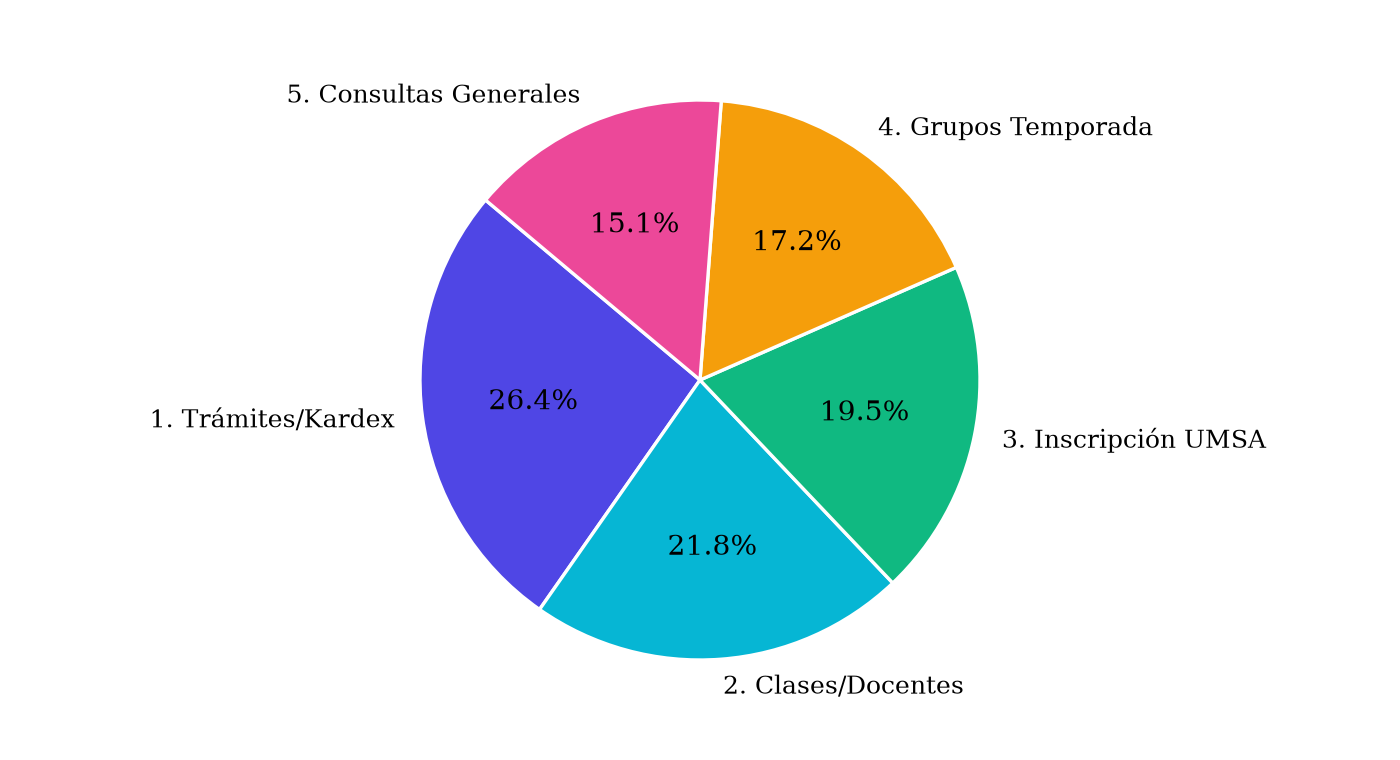
\includegraphics[width=0.7\textwidth]{prevalencia_topicos.png}
  \caption{Prevalencia de tópicos (documentos con tópico dominante).}
  \label{fig:topicos_prev}
\end{figure}

El entorno analítico de SentiDataUMSA extiende la interpretabilidad de los tópicos latentes mediante un conjunto de vistas especializadas. La Figura~\ref{fig:ui_lda_emociones} exhibe la configuración global de los cinco tópicos con sus distribuciones de probabilidad $\beta$ y el perfil afectivo asociado. En la Figura~\ref{fig:ui_topicos_mensajes} se muestra el muestreo empírico de mensajes reales anonimizados clasificados dentro de cada categoría temática desde Neon PostgreSQL. Asimismo, en la Figura~\ref{fig:ui_topicos_metricas} se detalla la matriz analítica de términos distintivos, pesos $\beta$ y puntuaciones Term-Score / TF-IDF por componente temático, mientras que la Figura~\ref{fig:ui_topicos_tiempo} proyecta la trayectoria temporal histórica (2018--2026) y el balance de carga afectiva de cada tópico.

\begin{figure}[htbp]
  \centering
  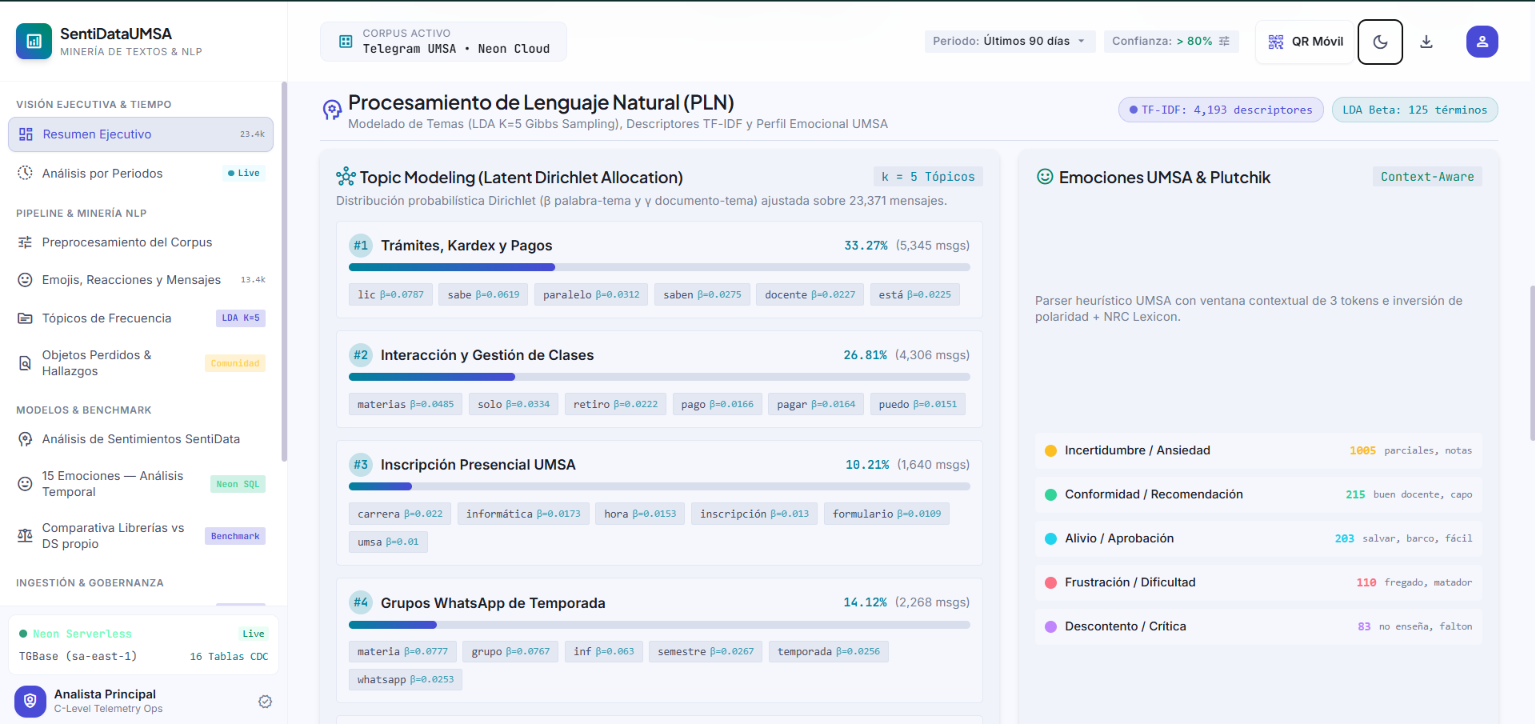
\includegraphics[width=0.90\textwidth]{figures/CAP3JNAC.png}
  \vspace{4pt}
  \caption{Estructura temática latente (LDA, $K=5$) y panel de emociones contextuales UMSA/Plutchik.}
  \label{fig:ui_lda_emociones}
\end{figure}

\begin{figure}[htbp]
  \centering
  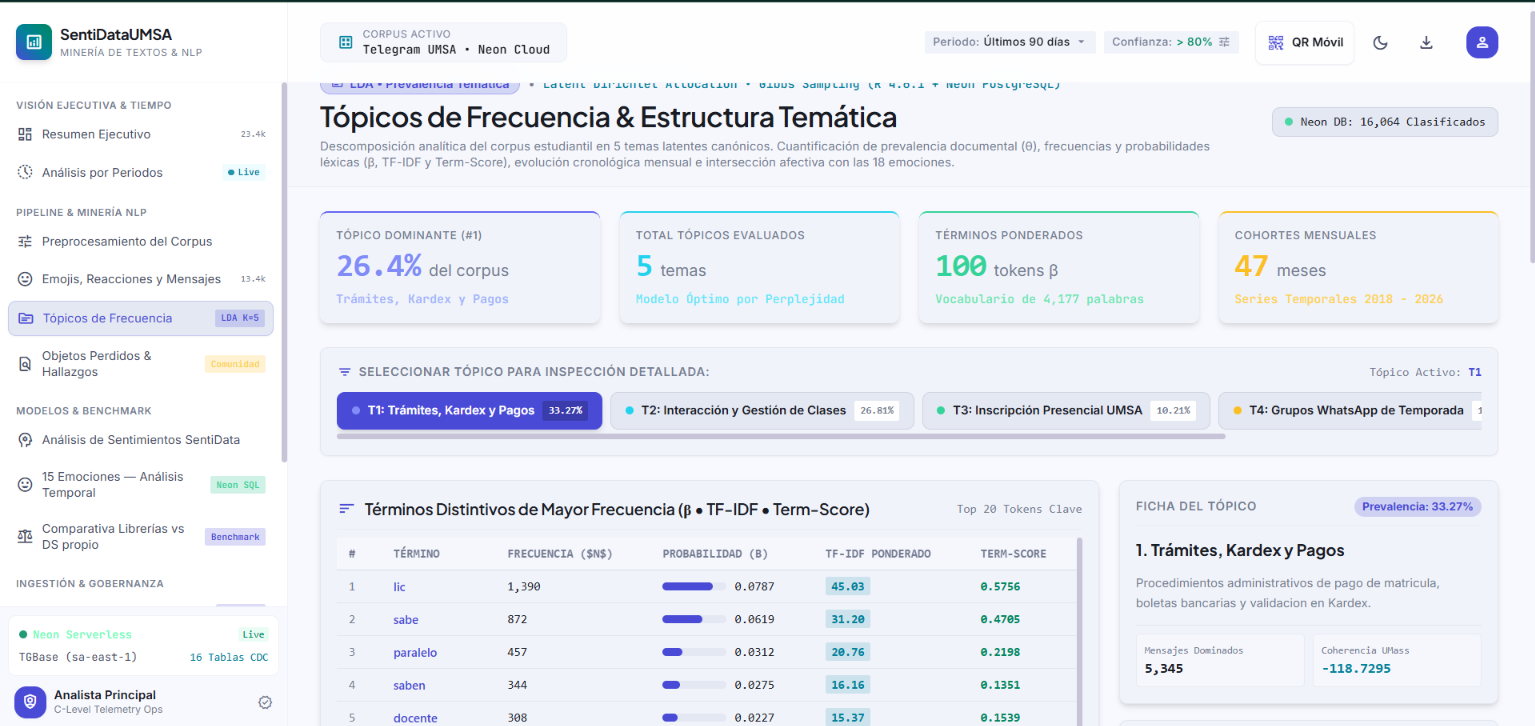
\includegraphics[width=0.90\textwidth]{figures/CAP12JNAC.png}
  \vspace{4pt}
  \caption{Muestreo empírico de mensajes reales anonimizados clasificados en el modelo temático en Neon PostgreSQL.}
  \label{fig:ui_topicos_mensajes}
\end{figure}

\begin{figure}[htbp]
  \centering
  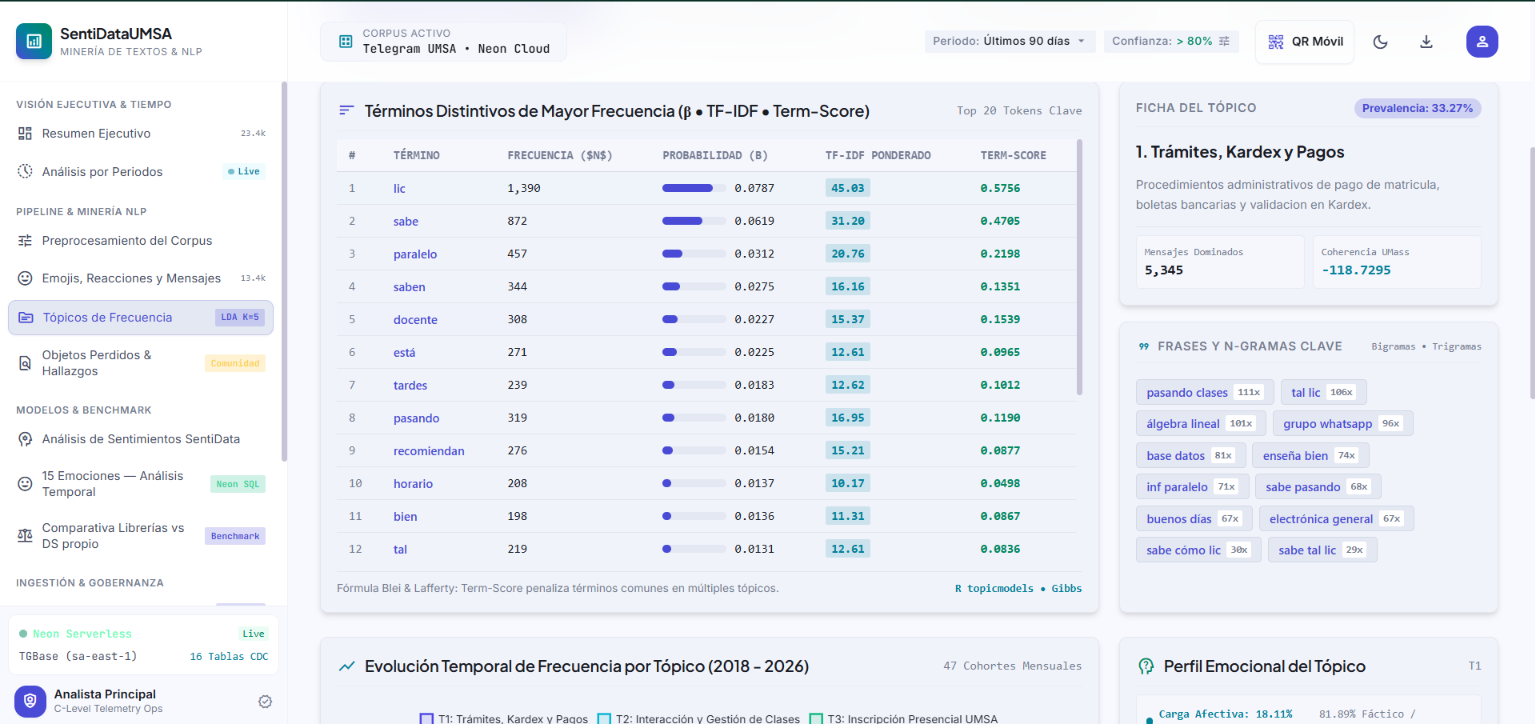
\includegraphics[width=0.90\textwidth]{figures/CAP13JNAC.png}
  \vspace{4pt}
  \caption{Matriz analítica de términos distintivos, pesos $\beta$ y ponderación Term-Score / TF-IDF por tópico.}
  \label{fig:ui_topicos_metricas}
\end{figure}

\begin{figure}[htbp]
  \centering
  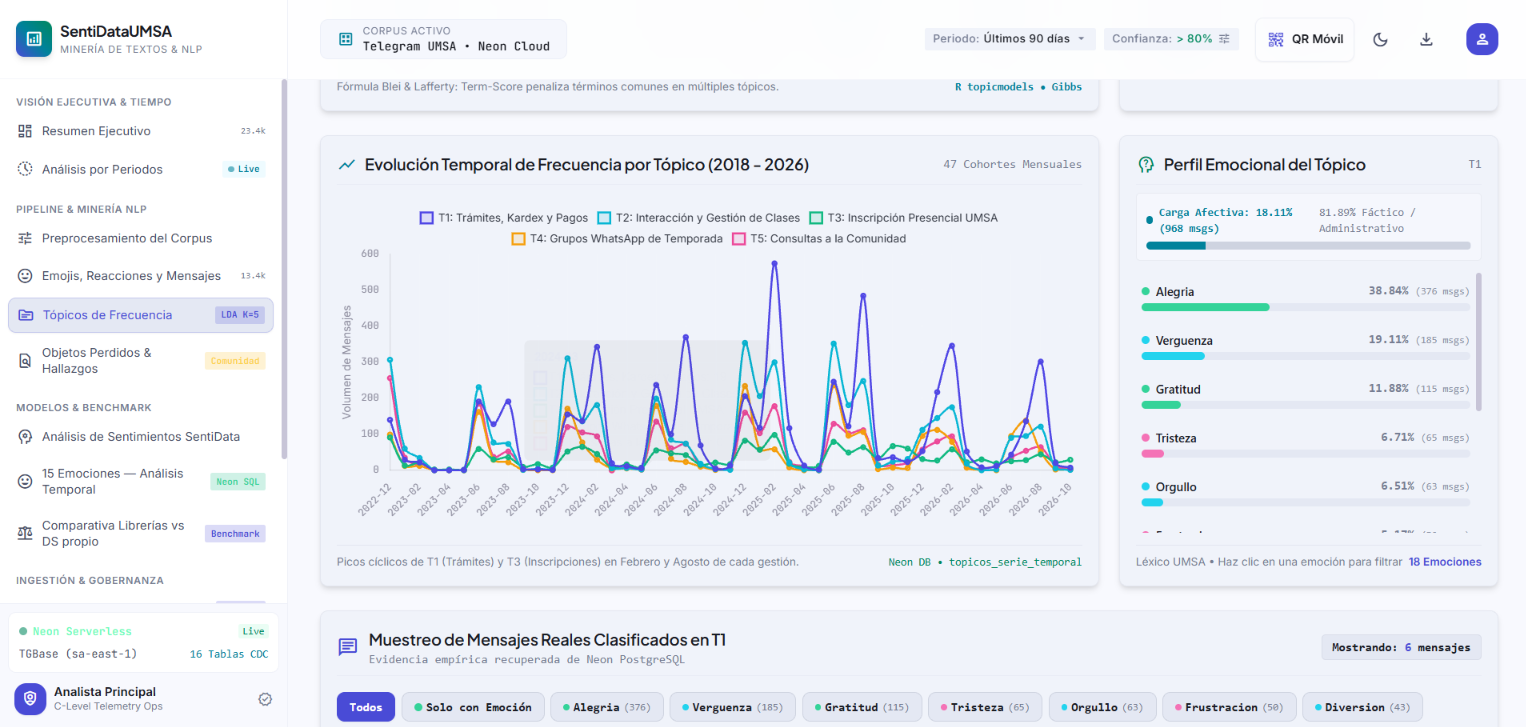
\includegraphics[width=0.90\textwidth]{figures/CAP14JNAC.png}
  \vspace{4pt}
  \caption{Trayectoria temporal de prevalencia temática (2018--2026) y perfil de carga afectiva del tópico.}
  \label{fig:ui_topicos_tiempo}
\end{figure}

\subsection{Transiciones de estado (cadenas de Markov)}
\label{sec:res-markov}

La quinta pregunta (PI5) aborda la dinámica entre estados. La
Figura~\ref{fig:markov} presenta la matriz de transici\'on estimada, donde cada celda
$(i,j)$ es la probabilidad de pasar del estado $i$ al estado $j$ entre mensajes
consecutivos. La diagonal está dominada por el estado neutro, lo que indica una fuerte
persistencia: la conversaci\'on tiende a permanecer en un régimen operativo.

\begin{figure}[htbp]
  \centering
  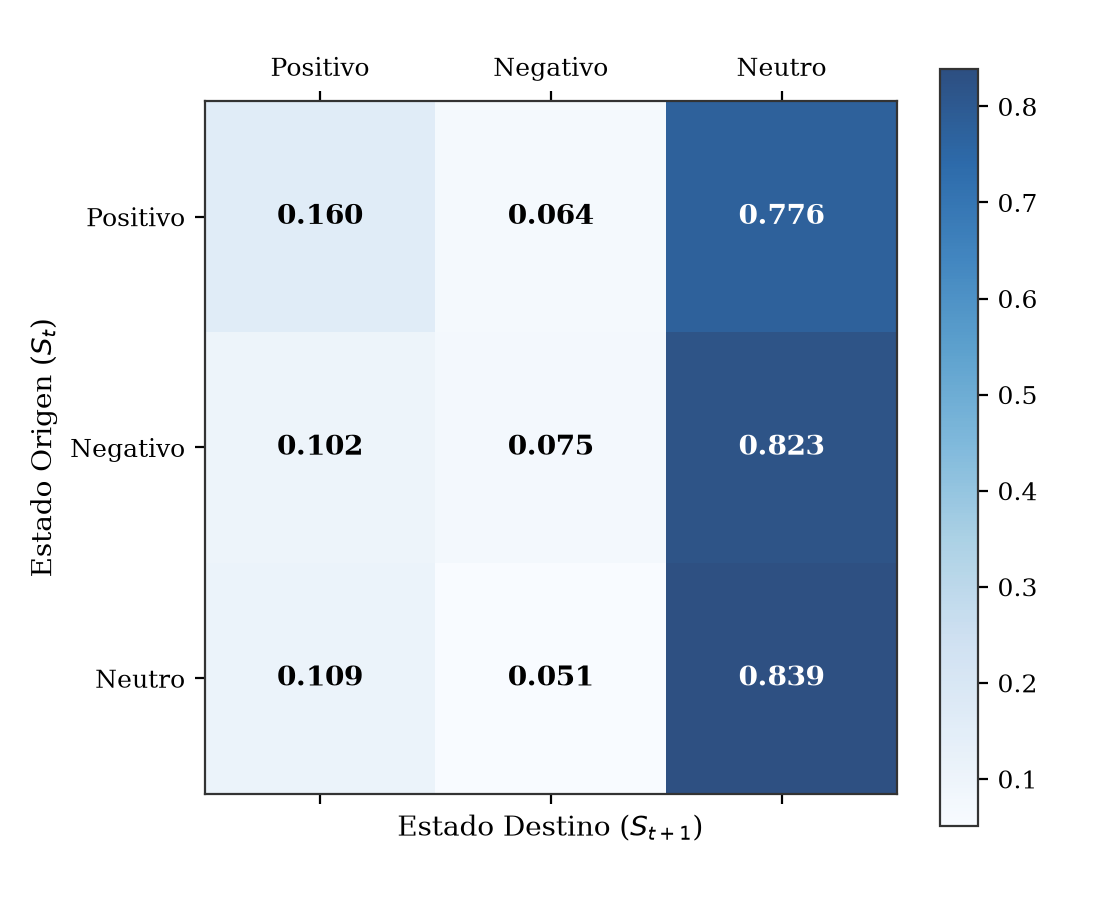
\includegraphics[width=0.62\textwidth]{transicion_markov.png}
  \caption{Matriz de transici\'on entre estados de polaridad.}
  \label{fig:markov}
\end{figure}

La Tabla~\ref{tab:markov} resume la distribuci\'on estacionaria $\pi$ y los tiempos
medios de permanencia. El estado neutro concentra \pctNeutro{}\% de la masa estacionaria,
frente a \pctPositivoEst{}\% del positivo y \pctNegativoEst{}\% del negativo. Los
tiempos de permanencia son elocuentes: \permanenciaNeutro{} turnos para el neutro,
frente a \permanenciaPositivo{} y \permanenciaNegativo{} para los estados con carga
afectiva. Los episodios negativos se disipan con relativa rapidez (recuperaci\'on media
de \recuperacionNegativa{} turnos), lo que sugiere una capacidad de recuperaci\'on del
clima conversacional.

\begin{table}[htbp]
  \centering
  \small
  \caption{Matriz de Probabilidades de Transición, Distribución Estacionaria y Tiempos de Residencia}
  \label{tab:transicion_markov}
  \label{tab:markov}
  \begin{tabular}{lcccccc}
    \toprule
    Estado & \multicolumn{3}{c}{Probabilidad de Transición hacia Estado Destino} & Distr. Estacionaria & T. Residencia \\
    \cmidrule(lr){2-4}
    Origen ($S_t$) & Positivo ($S_{t+1}$) & Negativo ($S_{t+1}$) & Neutro ($S_{t+1}$) & ($\pi_j$) & (turnos) \\
    \midrule
    Positivo & 0,160 & 0,064 & 0,776 & 0,115 (11,5\%) & 1,19 \\
    Negativo & 0,102 & 0,075 & 0,823 & 0,054 (5,4\%)  & 1,08 \\
    Neutro   & 0,109 & 0,051 & 0,839 & 0,831 (83,1\%) & 6,22 \\
    \bottomrule
  \end{tabular}
  \vspace{4pt}
  \begin{minipage}{0.94\textwidth}
    \footnotesize
    \textit{Nota.} Tiempo de recuperación ante episodios negativos: $\tau_{rec} = 1,08$ turnos. El análisis estocástico demuestra que el estado neutro/factual actúa como un atractor cuasi-absorbente dentro de la dinámica de conversación universitaria, absorbiendo más del 77\% de las transiciones salientes de los estados polares.
  \end{minipage}
\end{table}



\subsection{S\'intesis de hallazgos}

Los resultados convergen en un retrato coherente. El grupo es, ante todo, un espacio
operativo: la mayor parte de sus mensajes son informativos y no expresan afecto
expl\'\i{}cito, de ah\'\i{} la elevada proporci\'on de indeterminados. Cuando emerge
se\~nal afectiva, esta es predominantemente positiva y de carácter social
(\emph{\emocionTop{}}), aunque coexisten focos de ansiedad y frustraci\'on vinculados a
trámites y plazos. Temporalmente, la actividad sigue el calendario acad\'emico y la
dinámica de estados se caracteriza por la estabilidad del régimen neutro y la rápida
disipaci\'on de los episodios negativos.
